Now that you've integrated your concentrations with \acs{cmaq} it is
time to import them back into ArcGIS for evaluation.  As mentioned in
the introduction, \ioapi~files - the output format of \acs{cmaq} -
does not include standardized spatial georeferencing information, and
therefore will not display properly in ArcGIS.  Therefore, in order to
get around this we have developed an AQM Toolbox for ArcGIS with a
tool that can include \ioapi~files.

In short, this tool reads the custom attributes \ioapi~uses to record
spatial information and builds the spatial information to the file in
a more standard way\footnote{Specifically, the spatial information is
written using the \netcdf~CF Conventions.}.  The specific details of
this tool are documented in Appendix \ref{ioapi_tool_detail}.

Add this tool to your toolbox.  It has not yet been published to the
Esri Resources site, but it is included in the included
materials.  The tool should look as shown in figure \ref{ioapi_tool}.

\begin{figure}
	\centering
	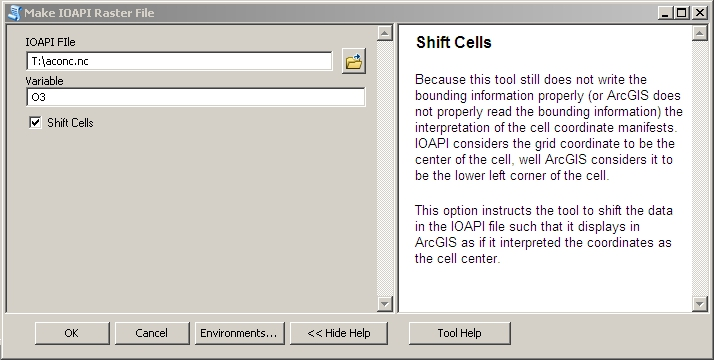
\includegraphics[width=0.6\textwidth]{fix_ioapi_tool.jpg}
	\caption{Example of \emph{Make IOAPI Raster File} tool}
	\label{ioapi_tool}
\end{figure}

Remember to enable Tool Help for details on the parameters.  For your
input \ioapi~file, choose an output file from your model that you
would like to display.  If you used \acs{cmaq}, you would likely want
to choose the \emph{ACONC} file.  For the variable, type the exact
name of your variable into this text box\footnote{You may need to open
your \netcdf~file with an application such as \emph{ncdump} to
retrieve your variable names.}.  Unlike the \emph{Make NetCDF
Raster Tool}, this tool is not able to read the variables from the
file.  Also, ensure that \emph{Shift Cells} is enabled.

You might notice that this tool has substantially fewer inputs as the
\emph{Make NetCDF Raster Tool}, this is partly due to the tool being
young, but also because the common use case this tool is expected to
be used for does not require the other inputs.

Press \emph{Ok}, your file is now having the spatial information
corrected and will then be added into your data frame as a raster
file.

If you still have the grids defined that were defined in section \ref{drawing_domains},
your data frame should resemble figure \ref{raster_loaded}.

\begin{figure}
	\centering
	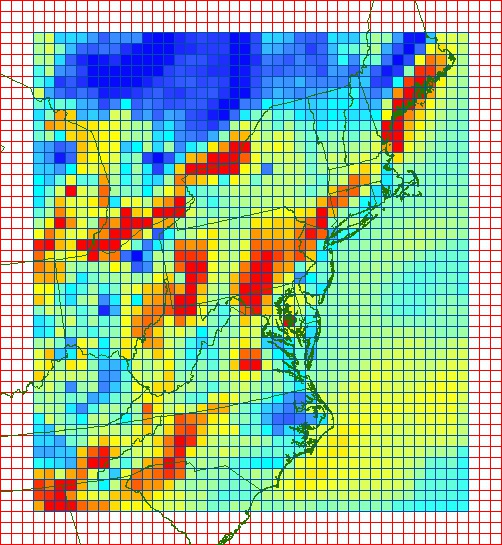
\includegraphics[width=0.6\textwidth]{raster_data_loaded.jpg}
	\caption{\ioapi~as raster file in ArcGIS.}
	\label{raster_loaded}
\end{figure}

Note that your time information has not been setup.  If you wish to
configure this, right click on your raster layer and open the
properties and choose the Time tab.  This is shown in figure
\ref{enable_time}.

\begin{figure}
	\centering
	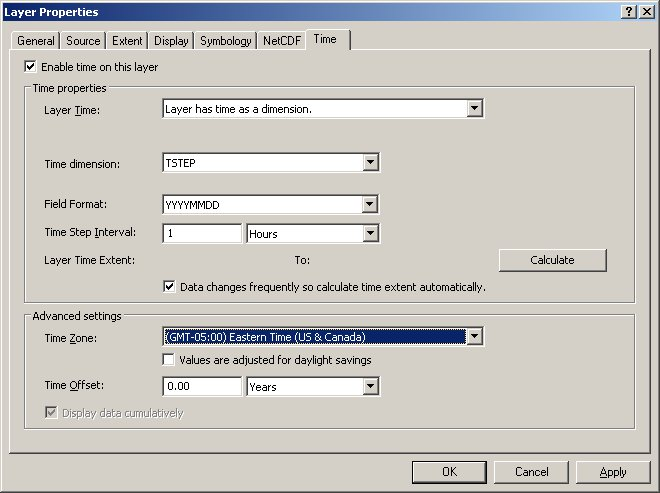
\includegraphics[width=0.6\textwidth]{enable_time.jpg}
	\caption{Enabling time information to a \netcdf~raster file}
	\label{enable_time}
\end{figure}

Now that time is added, you may now animate the layer.  This is
outside the scope of this learning module, however a tutorial for
animation can be accessed here:
\url{http://www.crwr.utexas.edu/gis/gishydro06/SpaceAndTime/NetCDF/Animating\%20netCDF\%20Data\%20in\%20ArcMap.htm}.
This tutorial also provides a secondary source for adding
\netcdf~files.
